\chapter{BIODATA PENULIS}
\begin{wrapfigure}{l}{0.3\textwidth}
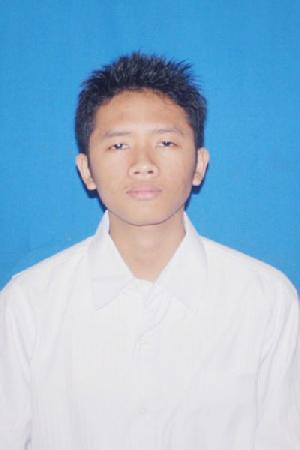
\includegraphics[height=0.3\textheight]{biodata/pas_foto.jpg}
\end{wrapfigure}

\textbf{Dewangga Winasforcepta Winardi}, lahir di Surabaya tanggal 18 Mei 1995. Penulis merupakan anak kedua dari 4 bersaudara. Penulis telah menempuh pendidikan formal TK Aisyiyah Bustanul Athfal Denpasar, SD Negeri 5 Ubung (2001-2007), SMP Negeri 5 Denpasar (2007-2010) dan SMA Negeri 4 Denpasar (2010-2013). Penulis melanjutkan studi kuliah program sarjana di Jurusan Teknik Informatika ITS. 

Selama kuliah di Teknik Informatika ITS, penulis mengambil bidang minat Algoritma Pemrograman (AP). Penulis pernah menjadi asisten dosen dan praktikum untuk mata kuliah Dasar Pemrograman (2015 dan 2016), Struktur data (2015 dan 2016). Selama menempuh perkuliahan penulis juga aktif mengikut kompetisi pemrograman tingkat nasional dan menjadi Juara 2 kategori pemrograman pada lomba COMPFEST Universitas Indonesia 2014. Selain itu penulis juga aktif di kegiatan organisasi dan kepanitiaan diantaranya menjadi staff Departemen Riset dan Teknologi HMTC ITS, wakil ketua National Programming Contest Schematics 2014, ketua National Programming Contest 2014, panitia Pemusatan Latihan Nasional 2 TOKI 2014, 2015, 2016 dan 2017 di ITS dan technical comitee Olimpiade Sains Nasional 2015 di Jogjakarta. Penulis dapat dihubungi melalui surel di \\ \texttt{dewangga.winardi@gmail.com}.
